\documentclass[a4paper,12pt]{article}

\usepackage{enumitem}
\usepackage[utf8]{inputenc}
\usepackage{textcomp}
\usepackage{xspace}
\usepackage[english,italian]{babel}
\usepackage[pdftex]{graphicx}
\usepackage{fullpage}
\usepackage{amsmath}
\usepackage{caption}
\usepackage{subcaption}
\usepackage{multirow}
\usepackage{amsfonts}
\usepackage{booktabs}
\usepackage{wrapfig}
%\usepackage[numbers]{natbib}

\usepackage{listings}
\lstset{
	basicstyle=\fontsize{10}{12}\ttfamily,
	inputencoding=utf8,
	language=C++,
	numbers=left,
	numberstyle=\tiny,
	tabsize=2,
	frame=single,
	backgroundcolor=\color{gray},
}

\setenumerate[2]{label=\alph*.}

\usepackage{color}
\definecolor{gray}{gray}{0.9}

\usepackage{hyperref}
\hypersetup{
	colorlinks=true
}
\usepackage{hypcap}

% qualche comando utile che evita di dover scrivere parole per intero
\newcommand{\boost}{boost\xspace{}}
\newcommand{\cpp}{C$++$\xspace{}}


% qualche comando per uniformare lo stile di scrittura
\newcommand{\shell}[1]{\texttt{#1}}
\newcommand{\code}[1]{\lstinline!#1!}

\begin{document}

\thispagestyle{empty}
\begin{center}
	\leavevmode
	\large
	\begin{tabular}{ r l }
		\multirow{2}{*}{
\includegraphics[width=2cm]{img/unipd_logo.png}} & \textsc{Università degli studi di Padova}\par \\
			& \textsc{Corso di laurea magistrale in Ingegneria Informatica} \\
	\end{tabular}
		
	\vfill
	{\Large Elaborazione di Dati Tridimensionali \par Relazione del progetto finale} \par
	\vskip .5cm
	\textbf{{\LARGE CNC Simulator}}\par
	\vskip 3cm
	\normalfont
	
	\begin{tabular}{ c c }
		\large Alberto \textsc{Franzin} & \large Nicola \textsc{Gobbo} \\
		\normalsize 1012883 & \normalsize 1014195 \\[1cm]
	\end{tabular}
	\normalfont
	\vskip 4cm
	
	\begin{flushright}
		\emph{Docente:}\\
		Prof. Emanuele \textsc{Menegatti}\\
	\end{flushright}

	
	\vfill
	{\large AA 2011-12}
\end{center}
\cleardoublepage


\begingroup
	\hypersetup{linkcolor=black}
	\setcounter{tocdepth}{2}
	\tableofcontents
\endgroup

\newpage

\section{Descrizione del problema}
Il progetto consiste nello scrivere un simulatore di macchina a controllo numerico (CNC - Computer Numerical Control) per il controllo della fresatura di un blocco di materiale.

Le specifiche fornite richiedono che il progetto sia eseguibile sia in ambiente Windows/Visual Studio che Linux. Viene anche fornito un diagramma con le principali classi da implementare, per uniformità. Viene richiesto che il simulatore accetti in ingresso un file contenente una lista di posizioni del blocco di materiale e dell'utensile di lavorazione, e la precisione della lavorazione, e che sia in grado di elaborare i movimenti comportati dalla lavorazione e di mostrare l'avanzamento della fresatura.



\section{Descrizione dei moduli implementati}
Sin dalle prime fasi della progettazione il programma è stato suddiviso in moduli, ognuno dei quali è implementato come una libreria, la quale comunica con le altre tramite interfacce fissate. Questa scelta è stata dettata sia dalla necessità di una efficace suddivisione del lavoro tra i programmatori che dalla volontà di rendere intercambiabili i moduli, per sostituirli con versioni più efficienti o debug-oriented.


\subsection{UML del moduli}
Per meglio comprendere le scelte progettuali fatte, viene presentato in figura \ref{fig:uml_cncsimulator} il diagramma UML dei moduli e delle classi principali che compongono il software.

\begin{sidewaysfigure}[htp]
	\centering
	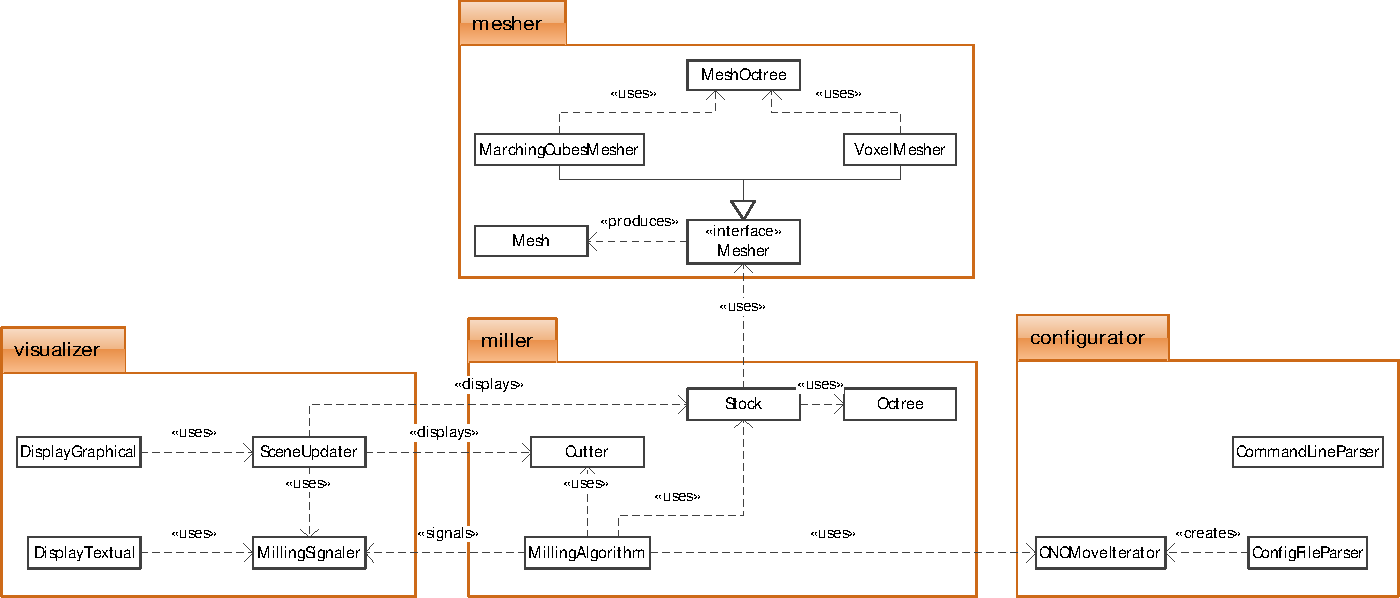
\includegraphics{img/uml_cncsimulator}
	\caption{UML dei moduli e delle classi principali del software.}
	\label{fig:uml_cncsimulator}
\end{sidewaysfigure}


\subsection{Configurator}
\code{configurator} è il modulo che si occupa di leggere i dati di ingresso e trasformarli in strutture dati comprensibili al resto del programma. Le fonti da cui attinge le informazioni sono la linea di comando, attraverso la classe \code{CommandLineParser}, e il file di configurazione, attraverso la classe \code{ConfigFileParser}.

\code{CommandLineParser} deve tutta la sua flessibilità nell'acquisizione della linea di comando alla libreria boost \code{program_options} di cui la classe è un semplice wrapper. Altro discorso va fatto per \code{ConfigFileParser}, classe scritta ad-hoc, in quanto il file da interpretare era di tipo \emph{plain-text} non strutturato. Per garantire una certa flessibilità al contenuto del file, questa classe permette di:
\begin{itemize}
	\item invertire la posizione delle sezioni \code{[PRODUCT]} e \code{[TOOL]}, fermo restando che la sezione \code{[POINTS]} deve rimanere l'ultima del file;
	\item gestire correttamente linee vuote o di commento, ovvero righe in cui il primo carattere non di spaziatura è ``\code{#}'';
	\item gestire parametri opzionali come la presenza o meno della direttiva \code{COLOR} nella sezione \code{[TOOL]}.
\end{itemize}
Individuata la sezione \code{[POINTS]}, \code{ConfigFileParser} demanda il compito di interpretare la lista delle posizioni a \code{CNCMoveIterator}. Questa classe estende \code{std::istream_iterator}, che a sua volta incarna il pattern \code{InputIterator}, proprio del \cpp: può perciò essere usata come un iteratore che, ad ogni dereferenziazione, legge la riga successiva del file e la interpreta come una coppia di roto-traslazioni, ritornando al chiamante queste informazioni con oggetti opportuni.

\subsubsection{Sviluppi futuri.}
L'implementazione della classe \code{ConfigFileParser} utilizza solo funzioni definite nello standard \cpp{}03 ma, nonostante questo, esistono delle incongruenze nella gestione dei file testuali da parte di Windows e Linux, dovute in primo luogo al diverso marcatore di fine riga dei due sistemi operativi. Queste incongruenze interessano per lo più la gestione dei parametri opzionali e, in ambiente Windows, portano ad una errata interpretazione del file di configurazione. Per evitare problemi di questo tipo ed aumentare la flessibilità della configurazione, si consiglia di separare in due documenti distinti quanto attualmente contenuto in uno unico: un primo file servirà a descrivere la configurazione della fresatura, codificata in formato XML, mentre il secondo conterrà la lista delle mosse che, dovendo essere letta in modo sequenziale, può mantenere l'attuale formato.

Un'ulteriore funzionalità non ancora implementata completamente è la gestione di cutter ``custom''. Le linee guida fornite non descrivevano nel dettaglio questo requisito, quindi l'ipotesi che è stata fatta riguarda da una parte l'apertura del codice rispetto all'aggiunta di nuovi cutter e, dall'altra, la possibilità di gestire mesh fornite dall'utente. Per quanto concerne l'introduzione di un nuovo modello di fresa, gli sforzi si sono rivolti a limitare le modifiche che andrebbero apportate alle classi esistenti; in merito alle mesh arbitrarie, invece, il \code{ConfigFileParser} dovrà venir modificato per accettare un ulteriore parametro opzionale nella sezione \code{[TOOL]}, il quale servirà a specificare il file contenente la mesh da visualizzare.


\subsection{Miller}
Il \emph{miller} è il componente che simula la fresatura vera e propria, verificando dove e come l'utensile della macchina compenetra il blocco di materiale, determinando la porzione da rimuovere e decidendo se sia o meno necessario attivare il getto d'acqua di pulitura.

Il prodotto da lavorare (classe \code{Stock}) e l'utensile (classe \code{Cutter}) sono i principali attori di questo modulo. Per gestire in maniera efficiente il processo di erosione lo stock è stato modellato con una particolare struttura dati chiamata \emph{octree}. Un octree è un albero di arietà 8 ---in questo caso, non bilanciato--- che, come si evince dalla figura \ref{fig:octree_explanation}, permette di segmentare uno spazio tridimensionale in regioni via via più piccole man mano che la aumenta la profondità. Ogni foglia rappresenta quindi un parallelepipedo di volume, detto \emph{voxel}, e su di essa è salvato un valore che identifica quali vertici sono stati asportati dal cutter e quali, invece, sono ancora presenti. Per motivi di performance a ciò si aggiungono le informazioni necessarie a calcolare le coordinate dei vertici stessi ed un collegamento alle strutture adibite alla visualizzazione grafica del blocco, come spiegato nella sezione \ref{sec:modules_mesher}.
\begin{figure}[htp]
	\centering
	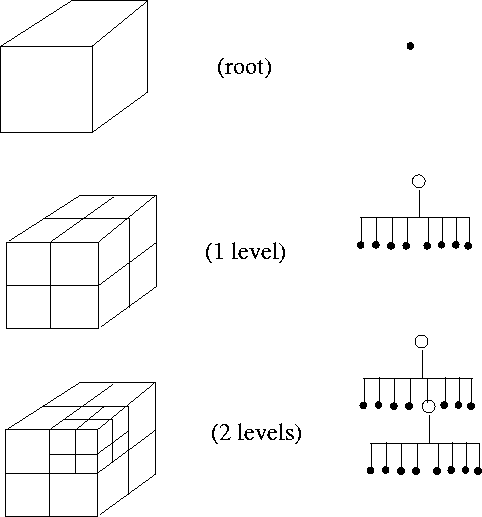
\includegraphics[width=.75\textwidth]{img/octree_explanation}
	\caption{Suddivisione dello spazio tridimensionale tramite albero octree. {\footnotesize (fonte immagine: \url{http://www.forceflow.be/wp-content/uploads/2012/04/octree1.gif})}}
	\label{fig:octree_explanation}
\end{figure}

All'interno del modulo di milling il cutter è caratterizzato da due soli parametri: una \emph{funzione di distanza} e una \emph{bounding box}. La funzione di distanza, descritta nell'equazione \eqref{equ:distance_function} indica se un punto dello spazio è interno o esterno all'utensile: nel caso sia interno, significa che è stato asportato.
\begin{equation} \label{equ:distance_function}
	distance(P) = 
		\begin{cases}
			< 0 & \text{se $P$ è esterno al cutter} \\
			\geq 0 & \text{se $P$ è interno al cutter}
		\end{cases}
	\qquad \text{ dove } P \in \mathbb{R}^3
\end{equation}
L'ingombro del cutter viene modellato attraverso un parallelepipedo orientato. La scelta di questa forma è dovuta al fatto che anche i voxel che costituiscono lo stock sono dei parallelepipedi: il problema dell'intersezione tra box è molto studiato in letteratura, e sono stati individuati algoritmi efficienti per questo tipo di verifica. L'orientamento, invece, serve a poter definire le più piccole dimensioni possibili tali da contenere il cutter: ciò permette di eseguire dei test di intersezione meno rapidi ma anche più accurati.

\subsubsection{Il processo di erosione.}
Per ogni ``mossa'' letta da file, il \emph{miller} converte le due rototraslazioni in una isometria tridimensionale del cutter nei confronti del sistema di riferimento del prodotto. L'algoritmo attraversa quindi l'octree per individuare tutti e soli i voxel che intersecano il volume di riferimento dello stesso cutter: i rami da percorrere sono scelti in base a diverse funzioni di intersezione che diventano via via meno precise, ma più veloci, via via che aumenta la profondità e, di conseguenza, il numero di voxel da analizzare. Giunto ad una foglia dell'albero, l'algoritmo ne enumera i vertici e, per ognuno di essi, invoca la funzione $distance$ del cutter: così facendo si marcano i punti interni alla superficie di taglio che, da quel momento in avanti, verranno considerati erosi.
Le foglie rimaste prive di vertici vengono quindi eliminate, mentre per le altre, se la profondità massima non è ancora stata raggiunta, l'algoritmo effettua una divisione in otto parti del volume di competenza, aggiungendo un nuovo livello all'albero. Come scelta progettuale si è deciso di non condividere i vertici comuni tra voxel contigui in quanto il concetto di vicinanza spaziale non viene modellato bene dalla struttura octree, soprattutto se sbilanciata. Il costo computazionale necessario a recuperare i voxel ``vicini'', infatti, sarebbe stato superiore ai vantaggi portati dalla condivisione dei vertici stessi. Al termine di ogni mossa, il \emph{miller} conteggia la quantità di materiale eroso e non ancora pulito e decide se attivare o meno il getto d'acqua: la scelta viene presa tramite una funzione a doppia soglia, caratterizzata da un ``rate di pulitura'', cioè dal volume di detriti che l'acqua riesce a pulire per ogni mossa.

Mostrare a video lo stato dell'erosione comporta uno scambio di informazioni tra \emph{miller} e \emph{mesher} in quanto questi due algoritmi operano in modo indipendente e con diversi tempi di elaborazione. Per gestire in maniera efficiente l'accesso concorrente ai dati, ogniqualvolta una foglia viene cancellata il \emph{miller} la inserisce in una lista opportuna mentre, per le foglie aggiunte o modificate, il percorso da esse alla radice viene evidenziato. Così facendo il processo di \emph{meshing}, dopo aver acquisito il controllo esclusivo dell'octree, potrà ricavare rapidamente tutte e sole le foglie modificate dalla sua ultima visita. Per impedire che il processo di \emph{milling} possa subire starvation dal \emph{mesher}, quest'ultimo viene attivato al più al termine di ogni mossa letta da file e, comunque, non più di 30 volte al secondo: nei casi reali il tempo di attesa forzata del \emph{miller} è ridotto in quanto, un ciclo di rendering impiega molto più tempo della simulazione di una singola posizione e quest'ultima è più lenta dell'attraversamento dell'albero sui percorsi evidenziati\footnote{I rapporti tra le durate delle operazioni indicate variano di molto in base alla profondità massima dell'albero e alla ``mobilità'' dell'utensile, ovvero al numero di voxel modificati ad ogni iterazione.}.

\subsubsection{Miglioramenti tentati e sviluppi futuri.}
Il processo di \emph{milling} è frutto di più riscritture successive, ognuna delle quali ha sperimentato un modo diverso per rendere più efficiente e veloce l'algoritmo. Il primo approccio scorreva l'albero per livelli sfruttando una coda come struttura dati di appoggio in cui inserire i nodi da analizzare. L'idea di fondo era facilitare la successiva parallelizzazione dell'algoritmo in cui vari thread avrebbero usato la coda per gestire i nodi da controllare, così come mostrato in figura \ref{fig:queue_parallel}.
\begin{figure}[htp]
	\centering
	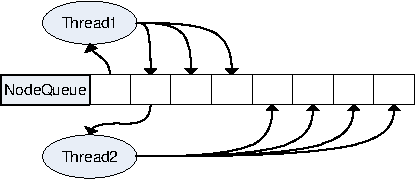
\includegraphics[width=.5\textwidth]{img/queue_parallel}
	\caption{Schematizzazione della prima idea di algoritmo parallelo che risolve il milling.}
	\label{fig:queue_parallel}
\end{figure}

Affrontare una simile strada avrebbe comportato un uso meno efficiente della memoria: l'inserimento dei nodi in una struttura dati in rapida espansione avrebbe comportato molti più accessi in RAM rispetto ad una semplice visita \emph{depth-first} in quanto la gerarchia di cache degli attuali elaboratori non sarebbe stata sfruttata appieno. La speranza era che il parallelismo riuscisse a sopperire a questo problema strutturale e, anzi, ad essere più rapido nell'esecuzione. Questo purtroppo non è avvenuto e, dai confronti con le implementazioni di altri colleghi, le prestazioni risultavano molto inferiori. Le ipotesi sulle motivazioni di questo ``fallimento'' sono state molteplici, ma la più plausibile risiede nell'aver scelto un approccio errato alla parallelizzazione, che male si adatta alla particolare struttura del problema: i nodi che devono venir analizzati sono molti ma, il lavoro da compiere su ognuno di essi è poco, per cui l'impianto necessario a gestire i thread introduce un overhead troppo elevato.

L'esperienza così maturata ha permesso di individuare un approccio migliore nella parallelizzazione del problema, analizzando l'octree attraverso il pattern Fork-Join\footnote{\url{http://www.oracle.com/technetwork/articles/java/fork-join-422606.html}} congiuntamente a uno thread-pool che permetta il \emph{work-stealing}. Così facendo si conservano tutti i vantaggi della visita \emph{depth-first}, senza relegare i thread all'analisi di singoli nodi, e beneficiando sia della possibilità di scrivere codice ricorsivo che di un processing embarassingly parallel.

Purtroppo per carenze di tempo e per la mancanza di librerie che implementano questo paradigma, si è optato per la classica versione ricorsiva. Questa risulta essere la più performante in single-thread ma, dal punto di vista dello spazio occupato, l'implementazione potrebbe essere ulteriormente migliorata, sfruttando i vantaggi offerti dalla ricorsione: attualmente, per esempio, ogni nodo dell'albero contiene un riferimento al padre, retaggio delle vecchie realizzazioni; questo puntatore può essere rimosso mantenendo comunque la possibilità di ``risalire'' la struttura dati durante il completamento delle chiamate ricorsive.



\subsection{Mesher}
\label{sec:modules_mesher}

Il mesher è il componente che, a partire dalla lavorazione effettuata dal miller, crea la mesh 3D dell'oggetto lavorato, traducendolo quindi in un oggetto tridimensionale da visualizzare.

Quando è pronto a eseguire del lavoro, richiede all’oggetto che rappresenta il prodotto le ultime modifiche effettuate: per tutte le foglie cancellate o aggiornate vengono eseguite le relative operazioni in maniera diretta, sfruttando il puntatore all’oggetto grafico contenuto;  quelle nuove, invece, vengono inserite nella scena solo se effettivamente visibili. Per facilitare il processo di visualizzazione, la parte di scena rappresentante il prodotto viene modellata con un octree le cui foglie contengono una molteplicità di voxel da rappresentare: questa scelta permette di ottimizzare l’uso delle risorse grafiche in quanto si diminuisce il numero di mesh, aumentandone la dimensione.

Il mesher esegue l'algoritmo Marching Cubes per creare la mesh a partire dai voxel. Marching Cubes permette inoltre di scartare dalla mesh quei voxel che sicuramente non sono visibili, perché totalmente interni o totalmente esterni (quindi eliminati) alla mesh.




\subsection{Visualizer}
Il visualizzatore è il componente che, interfacciandosi con l'utente, sincronizza gli altri moduli software e mostra i progressi dell'elaborazione in corso. Esso può operare in modalità grafica oppure testuale.

Nella modalità testuale il software si presenta come in figura \ref{fig:visualizer_textmode}, mostrando un riepilogo dei dati di configurazione e, nel caso sia stato lanciato ``in pausa'', attende che l'utente lo istruisca sul da farsi.
\begin{figure}[htp]
	\centering
	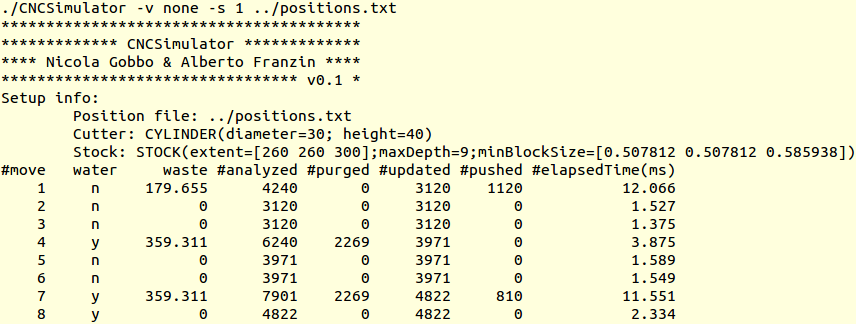
\includegraphics[width=.85\textwidth]{img/visualizer_textmode}
	\caption{\shell{CNCSimulator} avviato in modalità testuale.}
	\label{fig:visualizer_textmode}
\end{figure}

Durante l'esecuzione la modalità testuale stampa a video una nuova riga ad ogni ``mossa'' completata. Le informazioni ivi contenute riguardano il lavoro svolto dal \emph{miller} espresso in numero di foglie analizzate, aggiunte o cancellate, la quantità di materiale eroso, l'eventuale necessità di attivare il getto d'acqua e il tempo speso nell'elaborazione della mossa.

Il simulatore lanciato in modalità grafica esibisce una finestra simile a quella in figura \ref{fig:visualizer_graphicmode}. Oltre a mostrare lo stato dell'erosione in tempo reale permette all'utente di interagire con l'esecuzione in corso, mettendola in pausa, facendola avanzare di alcune mosse alla volta o disabilitando momentaneamente l'aggiornamento della scena per dedicare tutte le risorse hardware alla fresatura.
\begin{figure}[htp]
	\centering
	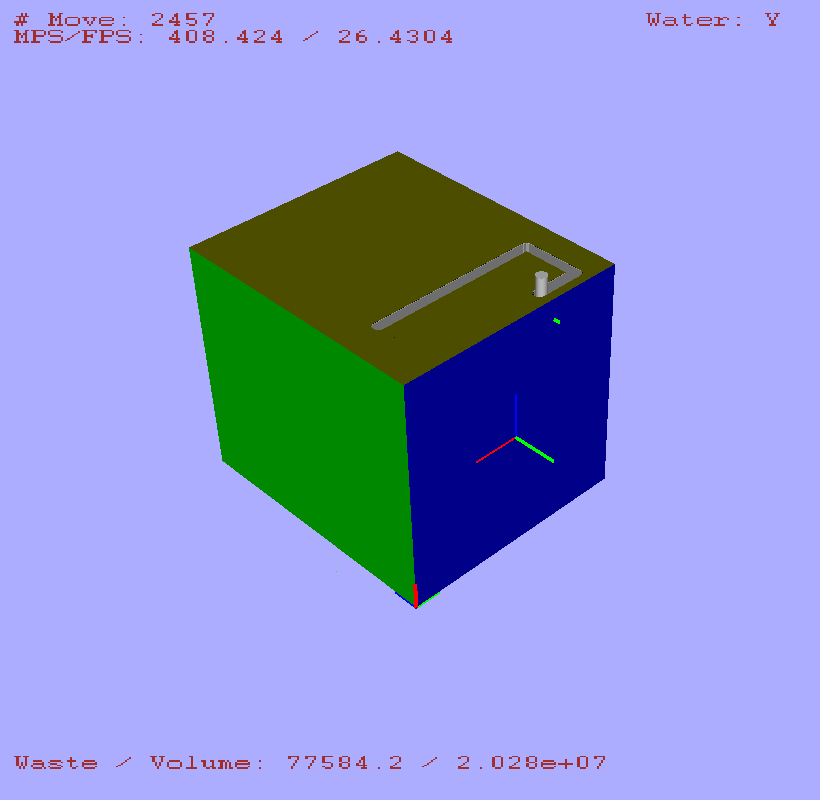
\includegraphics[width=.85\textwidth]{img/visualizer_graphicmode}
	\caption{\shell{CNCSimulator} avviato in modalità grafica.}
	\label{fig:visualizer_graphicmode}
\end{figure}

Come già detto il modulo \emph{visualizer} ha il compito di aggiornare la scena e per fare questo attende che il \emph{miller} completi almeno una mossa: questa attesa dura al più una quantità fissata di tempo, necessaria a garantire un numero di fotogrammi al secondo compreso tra 20 e 30. Nel caso in cui l'erosione venga completata in tempo, l'algoritmo procede ad aggiornare l'albero complessivo della scena richiedendo al cutter e allo stock le rispettive mesh -che verranno quindi riposizionate in base ai parametri della mossa corrente- e ricalcolando le varie quantità mostrate all'utente.


\section{Strumenti usati, prerequisiti e istruzioni}
\subsection{Strumenti usati}
Il progetto è stato sviluppato in \cpp. Per lo sviluppo in ambiente Linux abbiamo usato Eclipse su Ubuntu 12.04, mentre per l'ambiente Windows è stato usato Visual Studio 2010. Lo strumento usato per la compilazione è CMake ($\geq 2.6$).

\subsection{Prerequisiti}
Il progetto è stato sviluppato usando le seguenti librerie:
\begin{itemize}[noitemsep]
  \item Boost ($\geq 1.48$): è una libreria che fornisce diverse funzioni per molteplici scopi, come ad esempio gestione dei thread e gestione dei parametri.
  \item Eigen ($\geq 3.1.1$): è una libreria che mette a disposizione funzioni di algebra lineare;
  \item OpenSceneGraph ($\geq 3.0.0$): è un framework che permette di interfacciarsi alle librerie OpenGL in maniera semplificata ed efficiente \cite{osgbeginner}\cite{osgcookbook}.
\end{itemize}

\subsection{Istruzioni}
Il codice è disponibile all'indirizzo \url{http://code.google.com/p/edt-finalproject-nand/}.

Per compilare il progetto bisogna seguire i seguenti passi:
\begin{enumerate}
  \item portarsi nella cartella \verb!/path/del/progetto/!;
  \item lanciare il comando \verb!cmake flags source/CMakeLists.txt!, dove i \verb!flags! di compilazione possono essere:
    \begin{itemize}[noitemsep]
      \item \verb!-G"Visual Studio 10"! per la compilazione in ambiente Windows;
      \item \verb!-G"Unix Makefiles"! per la compilazione in ambiente Linux;
    \end{itemize}
    \begin{itemize}[noitemsep]
      \item \verb!-D CMAKE_BUILD_TYPE=Debug! per compilare in modalità \verb!debug!;
      \item \verb!-D CMAKE_BUILD_TYPE=Release! per compilare in modalità \verb!release!;
    \end{itemize}
  \item lanciare il comando \verb!make! per compilare.
\end{enumerate}

Per eseguire il progetto, lanciare il comando\\ \verb!/path/del/progetto/CNCSimulator opzioni file_positions!\\ dove:
\begin{itemize}
  \item le opzioni possono essere:
    \begin{enumerate}[noitemsep]
      \item \verb!-s x!, dove \verb!x! è la dimensione minima dei voxel. Minore è \verb!x!, maggiori saranno la precisione della simulazione e il tempo impiegato per completare l'esecuzione;
      \item \verb!-v box|mesh|none!, per specificare il tipo di visualizzazione, rappresentando i voxel come cubi (\texttt{box}), approssimando in maniera più precisa il taglio con l'algoritmo MarchingCubes (\texttt{mesh}) o in modalità solo testuale (\texttt{none});
      \item \verb!-p! lancia il simulatore in pausa;
      \item \verb!-f x!, dove \verb!x! indica il rate di apertura del getto d'acqua per la rimozione dei detriti in eccesso;
      \item \verb!-t x!, dove \verb!x! indica la quantità di materiale da rimuovere prima di attivare il getto d'acqua;
      \item \verb!-h!, per visualizzare il menu di help completo.
    \end{enumerate}
  \item \verb!file_positions! è il file contenente i movimenti da riprodurre.
\end{itemize}

In fase di esecuzione, è possibile modificare il comportamento del simulatore interagendo con esso mediante i seguenti comandi, visibili sul terminale premendo \texttt{h}:
\begin{itemize}[noitemsep]
  \item \verb'r'		esegue la simulazione alla massima velocità possibile, aggiornando il visualizzazore quando possibile;
  \item \verb'1'		aggiorna il visualizzatore ad ogni iterazione;
  \item \verb'2'		aggiorna il visualizzatore ogni $10$ iterazioni;
  \item \verb'3'		aggiorna il visualizzatore ogni $50$ iterazioni;
  \item \verb'p'		pausa;
  \item \verb't'		blocca/attiva gli aggiornamenti delle informazioni;
  \item \verb'k'		termina il milling;
  \item \verb'h'		mostra il menu di help;
  \item \verb'ESC'	esce dal simulatore.
\end{itemize}


\section{Esempi di lavorazione}
Mostriamo ora alcuni esempi di lavorazione, per vedere come i tempi di esecuzione catalogati variano a seconda dei parametri scelti.

Le prove sono state effettuate usando i due file messi a disposizione per i testing, chiamati \texttt{positions.txt} e \texttt{positions2.txt}. Il primo file contiene oltre $7000$ posizioni, e riproduce una fresatura limitata ad una ristretta porzione di blocco, generando quindi un Octree poco bilanciato. Il secondo file invece contiene oltre $20000$ posizioni e riproduce una fresatura che scava ``tutto attorno'' al blocco, generando un Octree più bilanciato, e risultando quindi più onerosa dal punto di vista computazionale. In figura \ref{tab:lavfinali} sono presentati gli esiti delle due lavorazioni.
\begin{table}[h]
	\centering
	\begin{tabular}{cc}
	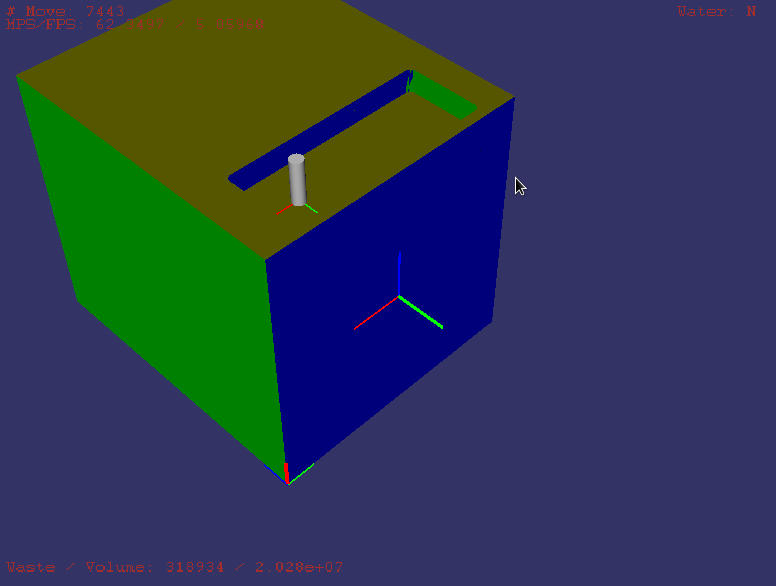
\includegraphics[width=0.48\textwidth]{img/screenshots/pos_box_v05_1.png} &%
	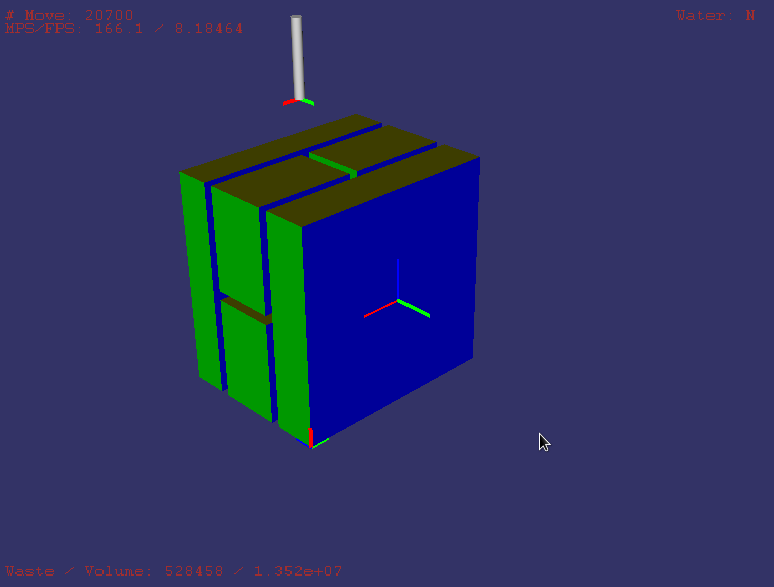
\includegraphics[width=0.48\textwidth]{img/screenshots/pos2_box_v1_2.png}\\
	\end{tabular}
	\caption{Risultato delle lavorazioni contenute nei file \texttt{positions.txt} e \texttt{positions2.txt}.}
	\label{tab:lavfinali}
\end{table}
I tempi riportati si riferiscono a test effettuati usando una macchina con Ubuntu Linux 12.04 a 64 bit, con processore Intel i7 a 1.73 GHz e 4GB di RAM, con il simulatore compilato in modalità \verb!release! e lanciato, salvo dove indicato, per completare la lavorazione alla massima velocità possibile. Per il profiling, invece, si è reso necessario compilare in modalità \verb!debug!. Per ciascuna configurazione sono state eseguite varie prove, le quali, una volta mediate, hanno prodotto i risultati qui presentati.

\subsection{Modalità testuale}
Vediamo innanzitutto (tabella \ref{tab:graphicsnone}) come si comporta il simulatore quando viene eseguito in modalità testuale.
\begin{table}[h]
	\centering
	\begin{tabular}{cccccc}
		\toprule
		& \multicolumn{2}{c}{file \texttt{positions.txt}} & & \multicolumn{2}{c}{file \texttt{positions2.txt}}\\
		\cmidrule(r){2-3}\cmidrule(r){5-6}
			\shortstack{Dimensione\\ Voxel} & \shortstack{Tempo \\\texttt{[s]}} & \shortstack{Memoria \\\texttt{[MB]}} & & \shortstack{Tempo \\\texttt{[s]}} & \shortstack{Memoria \\\texttt{[MB]}}\\
		\midrule
			3   & 0.517  & -     & & 2.446   & 22.7   \\
			2.5 & 0.543  & -     & & 2.558   & 12.2   \\
			2   & 1.632  & 17.2  & & 11.478  & 90.6   \\
			1.5 & 1.607  & -     & & 11.613  & 95.0   \\
			1   & 8.437  & 70.0  & & 99.785  & 463.4  \\
			0.5 & 67.691 & 334.7 & & 973.191 & 2764.8 \\
		\bottomrule
	\end{tabular}
	\caption{Riepilogo dei test effettuati in modalità testuale.}
	\label{tab:graphicsnone}
\end{table}
Con voxel grandi i tempi di esecuzione sono molto ridotti e molto simili, mentre con voxel più piccoli i tempi crescono compatibilmente con un fattore 8 (l'arietà dell'Octree). L'assenza di alcuni valori di memoria in tabella è causata dal fatto che la lavorazione contenuta nel file \texttt{positions.txt}, con voxel grandi, termina prima che sia possibile leggere la quantità di RAM occupata. Osservando però i valori rilevati per lo stesso file con voxel più piccoli, e paragonandoli con i valori osservati nella lavorazione riportata nel file \texttt{positions2.txt}, possiamo inferire che l'occupazione si limita a pochi \texttt{MB}. Da questo ragionamento si può dedurre che con voxel grandi l'albero generato è poco profondo e viene analizzato molto velocemente, con un impatto poco significativo sul tempo di esecuzione totale. Al diminuire della dimensione dei voxel, però, l'Octree diventa più profondo, e la sua scansione occupa una parte via via più consistente del tempo di esecuzione totale.

Per quanto riguarda i tempi rilevati per la lavorazione del file \texttt{positions2.txt} con dimensione voxel pari a $0.5$, si segnala che la lavorazione è stata rallentata dalle operazioni di swap causate dall'elevata quantità di memoria richiesta.

\subsection{Modalità grafica \texttt{box}}
La modalità grafica definita ``\texttt{box}'' non sfrutta  Marching Cubes per la rappresentazione dei voxel, ma rappresenta ciascuno di essi con un parallelepipedo. L'esecuzione caricherà quindi l'interfaccia grafica di OSG e al suo interno verranno visualizzate le varie fasi della lavorazione: il rendering, come detto, sarà basato su cubi di varie dimensioni che rappresentano i voxel dell'Octree.

\subsection{Modalità grafica \texttt{mesh}}
La terza modalità di visualizzazione è quella che utilizza l'algoritmo Marching Cubes per estrarre la mesh tridimensionale dai voxel. Come nella modalità \texttt{box}, anche in questo caso viene lanciato il visualizzatore di OSG, ma la lavorazione viene resa in maniera più precisa mediante l'approssimazione calcolata da Marching Cubes (vedasi sezione \ref{mcalgo}). Nella sezione successiva viene fatto un confronto tra le due modalità appena presentate.

\subsection{Confronto tra \texttt{box} e \texttt{mesh}}
Mettiamo ora a confronto la visualizzazione della lavorazione con la modalità di visualizzazione \texttt{box} e la modalità \texttt{mesh} (le immagini sono zoomate per apprezzare le differenze).
\begin{center}
\begin{table}[hbtp]
  \begin{tabular}{cc}
   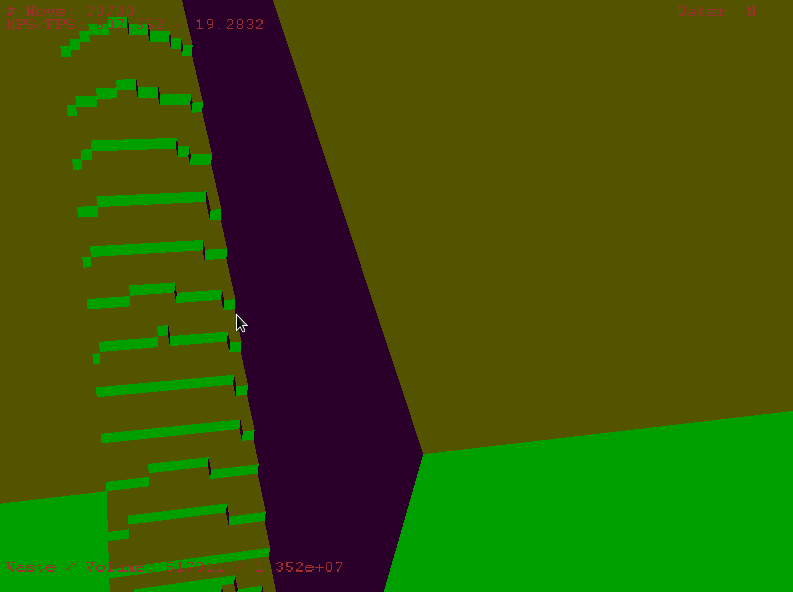
\includegraphics[width=0.48\textwidth]{img/screenshots/pos2_box_v2_2.png} &%
   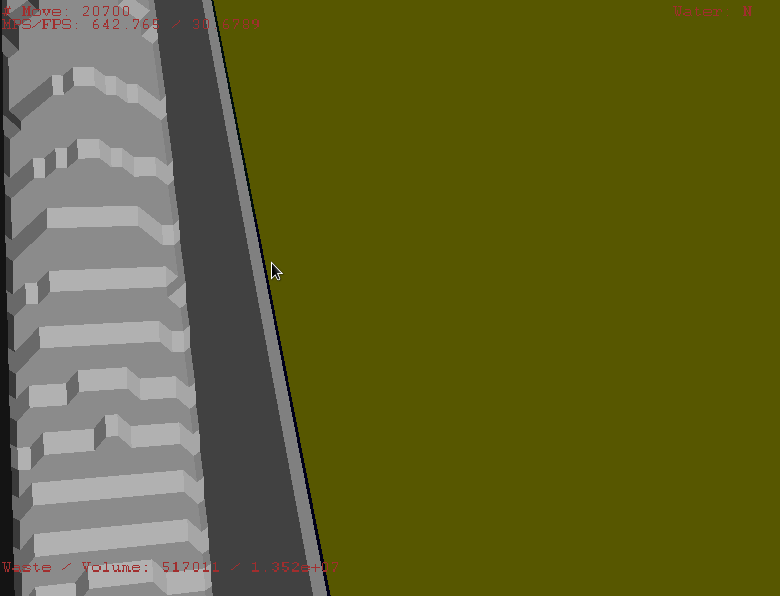
\includegraphics[width=0.48\textwidth]{img/screenshots/pos2_mesh_v2_2.png}\\
  \end{tabular}
  \caption{Confronto tra modalità \texttt{box} e modalità \texttt{mesh} con dim. voxel pari a $2$.}
  \label{tab:confrontobm1}
\end{table}
\end{center}

\begin{center}
\begin{table}[hbtp]
  \begin{tabular}{cc}
   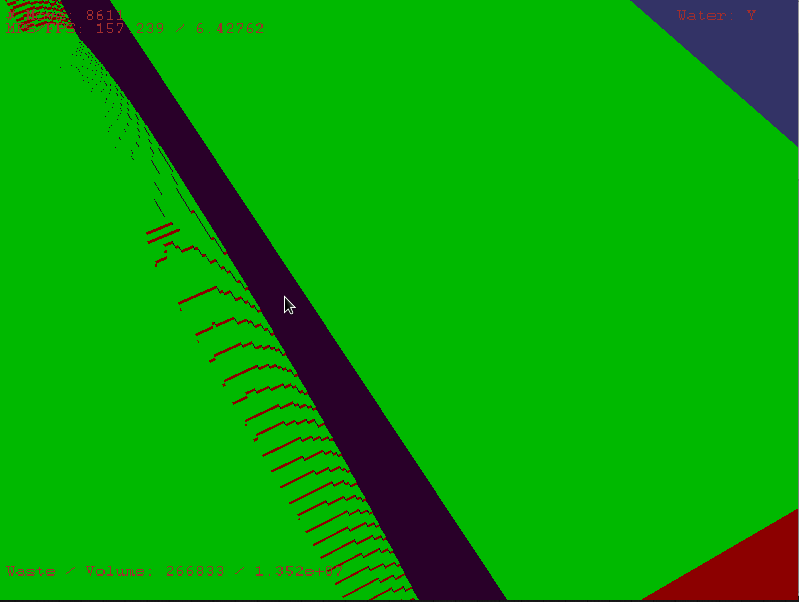
\includegraphics[width=0.48\textwidth]{img/screenshots/pos2_box_v1.png} &%
   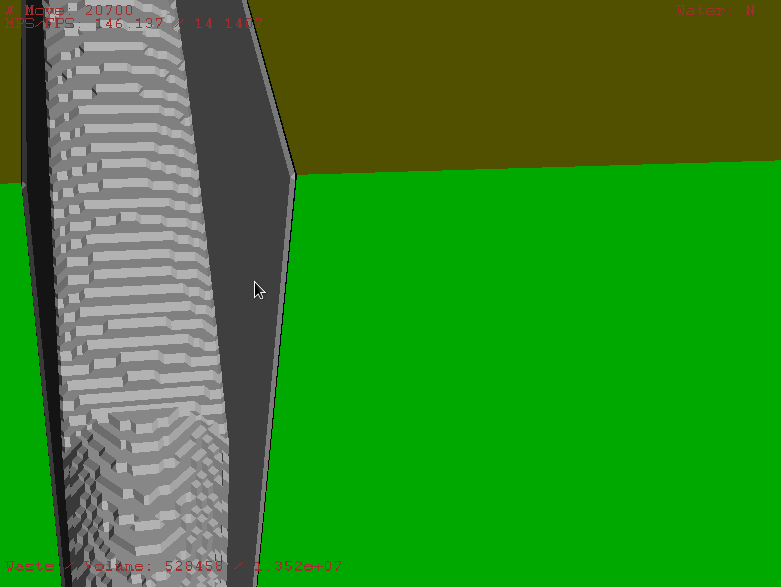
\includegraphics[width=0.48\textwidth]{img/screenshots/pos2_mesh_v1_2.png}\\
  \end{tabular}
  \caption{Confronto tra modalità \texttt{box} e modalità \texttt{mesh} con dim. voxel pari a $1$.}
  \label{tab:confrontobm2}
\end{table}
\end{center}

\begin{center}
\begin{table}[hbtp]
  \begin{tabular}{cc}
   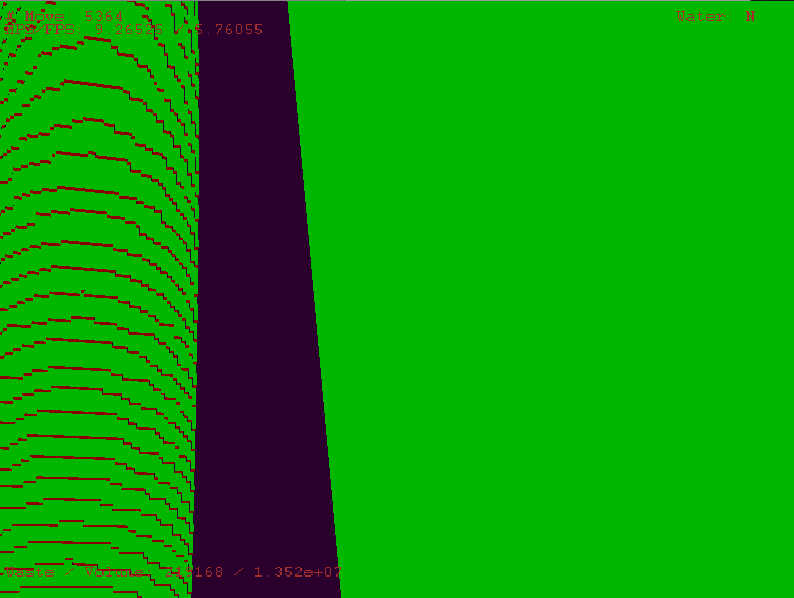
\includegraphics[width=0.48\textwidth]{img/screenshots/pos2_box_v05.png} &%
   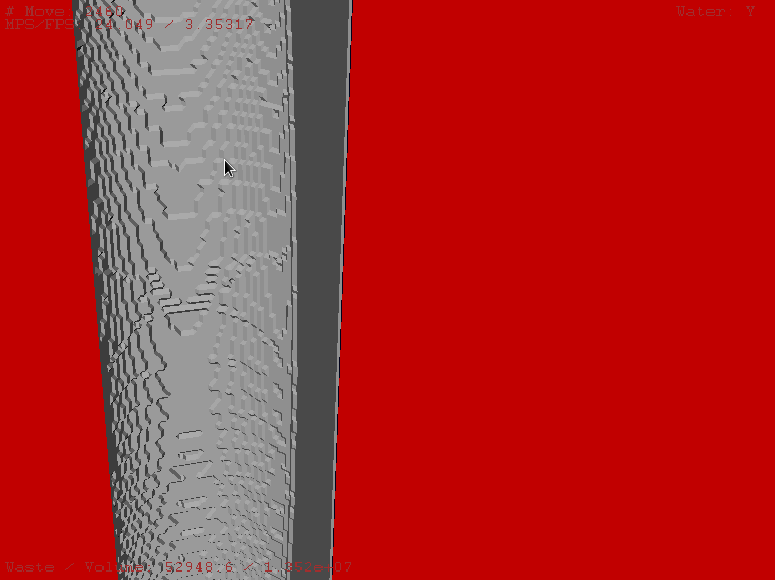
\includegraphics[width=0.48\textwidth]{img/screenshots/pos2_mesh_v05.png}\\
  \end{tabular}
  \caption{Confronto tra modalità \texttt{box} e modalità \texttt{mesh} con dim. voxel pari a $0.5$.}
  \label{tab:confrontobm3}
\end{table}
\end{center}

In \ref{tab:confrontobm1} vediamo la differenza nell'approssimazione della fresatura da parte del cilindro in modalità \texttt{box} (a sx) e \texttt{mesh} (a dx) con dimensione minima dei voxel pari a $2$. Vediamo come, nella modalità \texttt{mesh}, l'algoritmo Marching Cubes approssimi meglio la lavorazione, pur mantenendo visibile la struttura ``a cubi'' del rendering.

In \ref{tab:confrontobm2} e \ref{tab:confrontobm3} invece vediamo la stessa lavorazione, effettuata con dimensione dei voxel pari a, rispettivamente, $1$ e $0.5$. Via via che la dimensione dei voxel diminuisce, entrambe le modalità, ovviamente, approssimano in maniera sempre più precisa la fresatura. Tuttavia, mentre la modalità \texttt{box} approssima la lavorazione in modo sempre più preciso ma rimane comunque visibile la quadrettatura, l'algoritmo Marching Cubes che lavora alla stessa profondità dell'Octree fornisce risultati sempre più precisi e realistici.

Vediamo invece dalla tabella \ref{tab:confrontoBoxMesh} come l'implementazione con Marching Cubes possa risultare competitiva rispetto alla mera visualizzazione di cubi in lavorazioni brevi e che comportino la generazione di un Octree poco bilanciato e poco profondo. All'aumentare della profondità dell'albero, invece, la semplicità della generazione dei \texttt{Box} di OSG risulta più veloce. Per lavorazioni più complesse, che richiedono un Octree più completo, l'approccio \texttt{box} è più veloce rispetto alla generazione della \texttt{mesh} in tutti i test effettuati.

Segnaliamo che, per dimensioni minime dei voxel sufficientemente grandi, la lavorazione termina in tempi talmente brevi che risulta impossibile misurare un tempo attendibile. Inoltre, i tempi per le lavorazioni con Octree più profondo sono da considerarsi al netto del tempo di swap, che può essere più o meno consistente a seconda della quantità di memoria RAM a disposizione.

\begin{center}
  \begin{table}[hb]
   \centering
      \begin{tabular}{cccccc}
        \toprule
        & \multicolumn{2}{c}{file \texttt{positions.txt}} & & \multicolumn{2}{c}{file \texttt{positions2.txt}}\\
        \cmidrule(r){2-3}\cmidrule(r){5-6}
          \shortstack{Dimensione\\ Voxel} & \shortstack{Tempo \\con \texttt{box} \texttt{[s]}} & \shortstack{Tempo \\con \texttt{mesh} \texttt{[s]}} & & \shortstack{Tempo \\con \texttt{box} \texttt{[s]}} & \shortstack{Tempo \\con \texttt{mesh} \texttt{[s]}}\\
        \midrule
          3   & -      & -      & & 2.381    & 2.690    \\
          2.5 & -      & -      & & 2.510    & 2.581    \\
          2   & 2.090  & 1.988  & & 12.719   & 16.221   \\
          1.5 & 2.093  & 1.971  & & 12.581   & 19.051   \\
          1   & 10.267 & 9.807  & & 126.827  & 127.073  \\
          0.5 & 81.466 & 94.821 & & 1552.065 & 1684.734 \\
        \bottomrule
      \end{tabular}
      \caption{Confronto delle prestazioni tra modalità \texttt{box} e \texttt{mesh}.}
      \label{tab:confrontoBoxMesh}
  \end{table}
\end{center}

\subsection{Prestazioni grafiche}
Riportiamo ora (tabella \ref{tab:fps}) le prestazioni grafiche per le due modalità. Tali valori sono presi dai test effettuati sul file \texttt{positions.txt}, al termine della lavorazione. Il valore \texttt{max} nella colonna \texttt{\# mosse per aggiornamento} indica che il simulatore lavora alla massima velocità possibile, mentre negli altri casi il visualizzatore viene aggiornato dopo un numero fissato di passi.

\begin{center}
  \begin{table}[htbp]
   \centering
      \begin{tabular}{*{7}{c}}
        \toprule
          & & \multicolumn{2}{c}{\texttt{box}} & & \multicolumn{2}{c}{\texttt{mesh}}\\
        \cmidrule(r){3-4}\cmidrule(r){6-7}
          \shortstack{Dimensione \\Voxel} & \shortstack{\# mosse per\\aggiornamento} & MPS & FPS & & MPS & FPS \\
        \midrule
          3   & max      & 14866.3      &  1.99735  & & 14301.8      &  1.92151     \\
          3   & 50       & 883.677      &  40.1294  & & 1181.59      &  47.3080     \\
          3   & 10       & 309.825      &  57.1947  & & 294.285      &  55.3144     \\
          3   & 1        & 15.7666      &  30.4380  & & 19.3040      &  32.8477     \\ \\
          2   & max      & 4782.33      &  3.21263  & & 4591.99      &  35.1164     \\
          2   & 50       & 1091.91      &  32.2764  & & 1232.29      &  48.8411     \\
          2   & 10       & 302.094      &  43.5912  & & 313.589      &  57.7210     \\
          2   & 1        & 21.9418      &  31.2309  & & 17.6811      &  31.7073     \\  \\
          1   & max      & 790.810      &  5.41869  & & 811.415      &  27.6904     \\
          1   & 50       & 562.534      &  13.7240  & & 584.776      &  35.4339     \\
          1   & 10       & 160.020      &  19.2419  & & 276.251      &  46.4686     \\
          1   & 1        & 16.8491      &  20.1293  & & 21.0637      &  32.6215     \\ \\
          0.5 & max      & 87.5204      &  2.22240  & & 76.4261      &  7.04729     \\
          0.5 & 50       & 61.7659      &  6.52264  & & 78.0658      &  8.25444     \\
          0.5 & 10       & 47.7159      &  5.91720  & & 62.8882      &  10.8912     \\
          0.5 & 1        & 6.01965      &  7.00878  & & 12.8600      &  14.8038     \\
        \bottomrule
      \end{tabular}
      \caption{Framerate in modalità \texttt{box} e \texttt{mesh}.}
      \label{tab:fps}
  \end{table}
\end{center}

Analizzando i risultati ottenuti, notiamo come per profondità dell'Octree non troppo elevate, la lavorazione al massimo della velocità possibile penalizzi le prestazioni del visualizzatore, pur mantenendole più che buone. I FPS sono costantemente sopra i $25$, ad eccezione della lavorazione alla velocità massima con Octree poco profondo: tuttavia, come già abbiamo avuto modo di notare analizzando i tempi di esecuzione, i test effettuati in queste condizioni sono poco significativi, in quanto la lavorazione termina troppo presto per avere valori realistici. Vediamo infatti come il numero di movimenti al secondo sia circa il doppio delle mosse realmente eseguite, e il visualizzatore, sostanzialmente, si apre a lavorazione conclusa.

Vediamo inoltre come l'aggiornamento ogni $10$ posizioni dia risultati migliori, in termini di FPS, rispetto agli altri (quando disponibile, ogni $50$, ogni aggiornamento). Infine, è interessante notare come la visualizzazione in modalità \texttt{mesh} comporti una visualizzazione più rapida rispetto alla modalità \texttt{box}, a parità di parametri. Questo è probabilmente indice di una migliore gestione da parte di OpenSceneGraph delle figure costituite da semplici poligoni rispetto ai \texttt{Box}, che sono oggetti più pesanti, tale da compensare anche l'overhead dovuto a Marching Cubes.

Per dimensione dei voxel pari a $0.5$ invece si osserva come la lavorazione diventi talmente onerosa da penalizzare in maniera consistente anche l'aggiornamento della scena video: le prestazioni del rendering quando l'Octree è molto profondo sono infatti le peggiori. Probabilmente potrebbero essere migliorate sfruttando le librerie Cuda, che noi non abbiamo usato non avendo a disposizione una scheda grafica nVidia.

\subsection{Carico relativo dei moduli}
Analizziamo infine cosa succede \textit{all'interno} di un'esecuzione del simulatore. Per farlo, osserviamo il grafico delle chiamate in figura \ref{fig:callgraph}. Questo grafico è stato ottenuto a partire dal una lavorazione in modalità \texttt{mesh} con dimensione dei voxel pari a $2$, con gli strumenti di debug e profiling \texttt{valgrind}, \texttt{callgrind} e \texttt{kcachegrind}.

\begin{figure}[htp]
	\centering
	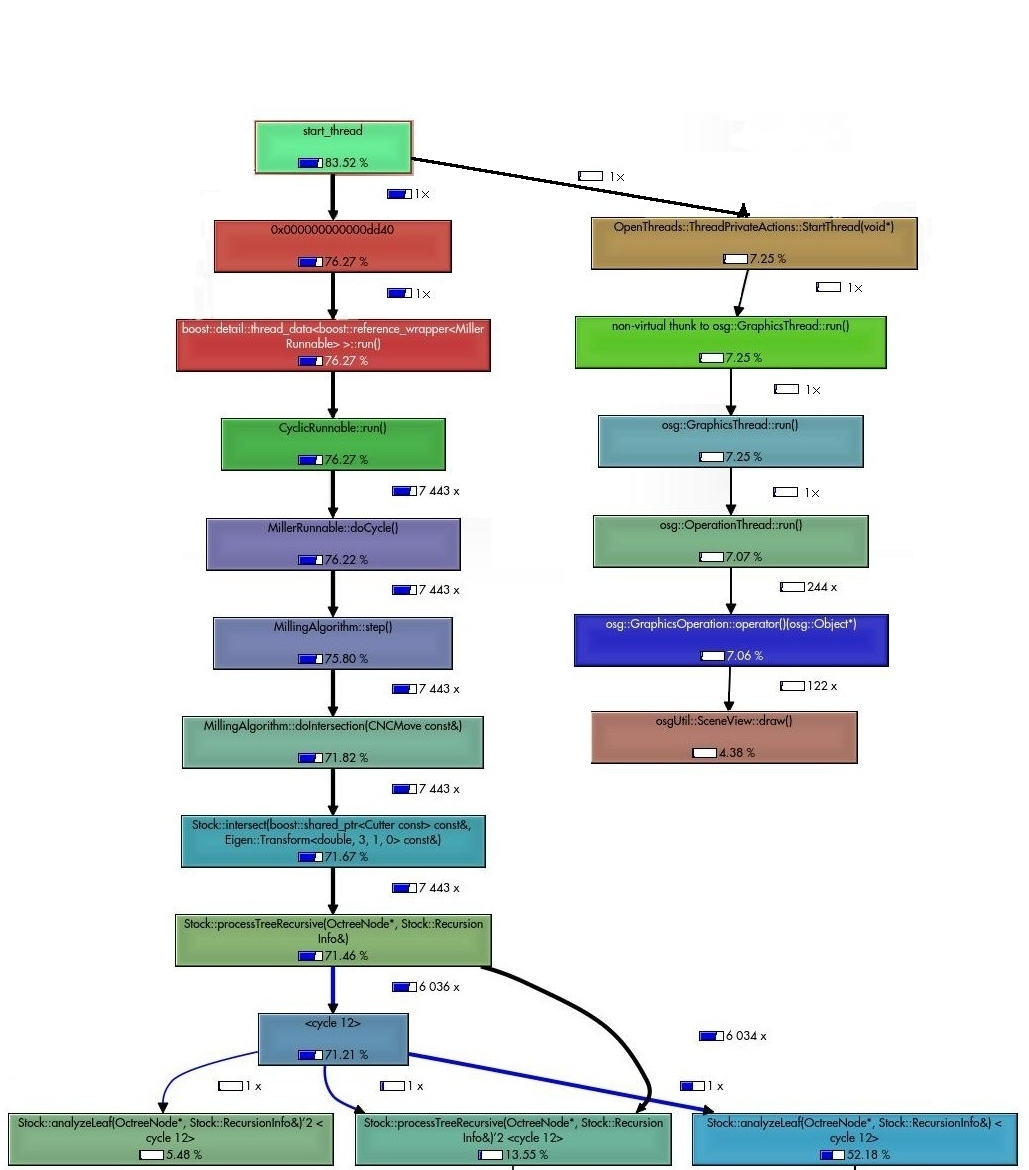
\includegraphics[width=.97\textwidth]{./img/callgraph.jpg}
	\caption{Grafico delle chiamate del simulatore.}
	\label{fig:callgraph}
\end{figure}

Il modulo che lavora per la maggior parte del tempo è chiaramente il Miller, che consuma circa i 3/4 di cicli processore impiegati in totale. Il metodo \texttt{CyclicRunnable::run()} chiama infatti \texttt{MillerRunnable::doCycle()} per 7443 volte, ovvero il numero di iterazioni dell'algoritmo di milling. Questa è chiaramente l'operazione più onerosa eseguita dall'algoritmo, e quella in cui si dovrebbero concentrare eventuali sforzi di ottimizzazione per ottenere un prodotto più performante.

La visualizzazione grafica, che inizia con l'invocazione del metodo \texttt{Display::draw()} è invece responsabile del 15\% circa del tempo di calcolo.

Per quanto riguarda i rimanenti moduli, se il configuratore viene eseguito solo preliminarmente alla lavorazione e con compiti di setup, e ci aspettiamo quindi un impatto limitato sul tempo totale, notiamo invece come in questa prova il Meshing sia assente dal grafo, segno di come anche il suo impatto sia limitato rispetto al Milling, conseguenza dell'efficienza dell'algoritmo Marching Cubes e della bontà della sua implementazione. Segnaliamo tuttavia come questo accada con dimensione minima dei voxel pari a 2: diminuendo la dimensione dei voxel l'impatto dovuto a Marching Cubes aumenta notevolmente, quindi ci aspettiamo di veder comparire anche i metodi del Mesher tra quelli più impattanti sul tempo. Tuttavia, questi test non sono stati effettuati, in quanto l'esecuzione di \texttt{callgrind} rallenta di molto il tempo di esecuzione della simulazione, e una run con voxel più piccoli avrebbe richiesto con ogni probabilità diverse ore prima di giungere al termine.

Come si può facilmente evincere dai risultati appena presentati, i metodi che vengono maggiormente invocati sono quelli che permettono l'interazione tra cutter e Octree. Il metodo in assouto più chiamato è infatti \texttt{CylinderCutter::getDistance()} che misura la distanza tra il cutter (che in tutti i test effettuati era appunto di forma cilindrica) e il voxel più vicino, per determinare se c'è intersezione e quindi rimozione di materiale. Segue, con circa metà invocazioni, la gestione degli smart pointers di Boost e, con poco più di un terzo di chiamate, il metodo \texttt{Stock::IntersectionTester::fastInt()} che esegue i calcoli per determinare se c'è intersezione tra cutter e voxel.


\section{Conclusioni}
Il simulatore mostra come procede passo dopo passo il lavoro di fresatura, permettendo di regolare precisione della lavorazione e del rendering e la velocità di visualizzazione.

Con i file di esempio messi a disposizione, le operazioni vengono portate a termine correttamente e con buone prestazioni, nonostante non sia stato possibile sfruttare CUDA perché nessuno di noi ha a disposizione una scheda grafica Nvidia.


% %aggiunge la bibliografia all'indice
 %%niente sezioni anche qui, ovvio....
\clearpage

% \bibliographystyle{plain}
% \bibliography{biblio}
% \addcontentsline{toc}{section}{Bibliografia}

\end{document}
